\documentclass[12pt]{article}

% Packages
\usepackage[utf8]{inputenc}
\usepackage{multicol}
\usepackage{amsmath}
\usepackage{graphicx}
\usepackage{hyperref}
\usepackage{booktabs}
\usepackage{hyperref}
\usepackage[left=0.7in,right=0.7in,top=1in,bottom=1in]{geometry} % Set margins

% Document settings
\title{Analysis of Bat Frequencies for Classification of Species using Machine Learning Algorithms}
\author{Hoang Nguyen}
\date{\today}

\begin{document}

\maketitle

\section{Introduction}
    \text Bats are fascinating creatures because they utilize echolocation to navigate around. In this report, I analyze the sound of an unknown bat using digital signal processing to understand the frequency domain features, ultimately revealing interesting properties that bats possess while navigating their surrounding environments. The study explores the ultrasound signal's frequency-domain characteristics by using Fourier transforms to identify distinct frequency peaks, thereby shedding light on the harmonic nature of bat ultrasound. Furthermore, performing a spectrogram analysis can help identify the bat's frequencies, which is $\sim10.157\,\text{kHz}$. Additionally, this particular species of bat possesses such high frequency that it is too difficult to be visible on the time-domain plot, a frequency-shifting technique can be used to visualize the oscillations, thus providing better insights. Ultimately, these insights can be used to identify unknown bat species by classifying various bat species in nature using Support Vector Machines (SVM) and Random Forests.
    
\section{Analysis and Discussion}
\subsection{Loading the Audio File (Q 3 - 1)}
The shape of the audio array is given by $(7872, 2)$, which signifies that the audio file is a stereo recording with two distinct channels, each having $7872$ samples. This stereo format, composed of left and right channels, is commonly used in audio recordings to create a spatial sound experience. Especially in recording bat ultrasound, then the recording equiment is highly sensitive for detecting intricate signal. However, for the purposes of this analysis, one of the two channels is selected to attain a mono audio signal. The shape of this mono audio array is $(7872,)$, reflecting the single-channel nature of the data with $7872$ audio samples.

\subsection{Time-Domain Signal Analysis (Q 3 - 2)}
After loading the audio file of a bat sound and selecting one of its channels, a time-domain plot of the signal was generated. The plot provides a visual representation of how the amplitude of the signal varies over time.

\begin{figure}[h]
\centering
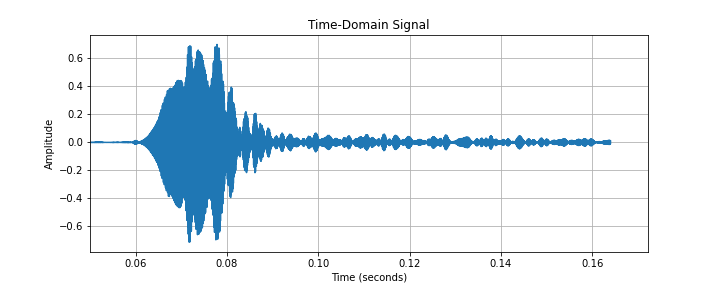
\includegraphics[width=1.0\textwidth]{time_domain_signal_plot.png}
\caption{Time-domain plot of the bat sound signal.}
\end{figure}

From this time-domain plot of the bat sound signal, several key numeric characteristics are:

\begin{itemize}
    \item \textbf{Signal Duration:} The total duration of the signal, as represented on the x-axis. Here the signal is focused mainly from the moment the bat begins generating the sound, which is about 0.06 seconds into the audio. The sound is approximately 0.04 seconds (from 0.06 to 0.1 seconds). This duration is typical for a single echolocation call or a series of calls from a bat. But from the graph of the time-domain signal, this is likely a single echolocation call.
    
    \item \textbf{Amplitude Range:} The amplitude of the signal varies across a range of -0.65 to 0.65, indicating the varying intensity of the echolocation calls. The peak amplitudes might correspond to the closest approach of targets or the most intense phase of the echolocation.
    
    \item \textbf{Characteristic Patterns:} At around 0.65 to 0.75 seconds, the plot shows a distinctive pattern where the amplitude sharply peaked at 0.65. This could represent a specific behavior, such as targeting prey or navigating around obstacles.
    
    \item \textbf{Noise and Variability:} The plot exhibits a degree of noise and variability through out the whole audio, it is especially noticeable in sections beyond 0.08 seconds after the bat generates the sound. These could be due to environmental factors, the inherent nature of the bat's echolocation mechanism or the recording equipment itself.

\end{itemize}

\subsection{Fourier Transform and Spectrum Analysis (Q 3 - 3)}
The time-domain plot, however, doesn't provide much insight into the frequency of this species of bat. So, analyzing the Fourier transform of the bat signal can give much better insights into the characteristics of the bat sound. After performing Fourier transformations and calculating the modulus the the sound, interesting properties are observed as followed:

\begin{figure}[h]
\centering
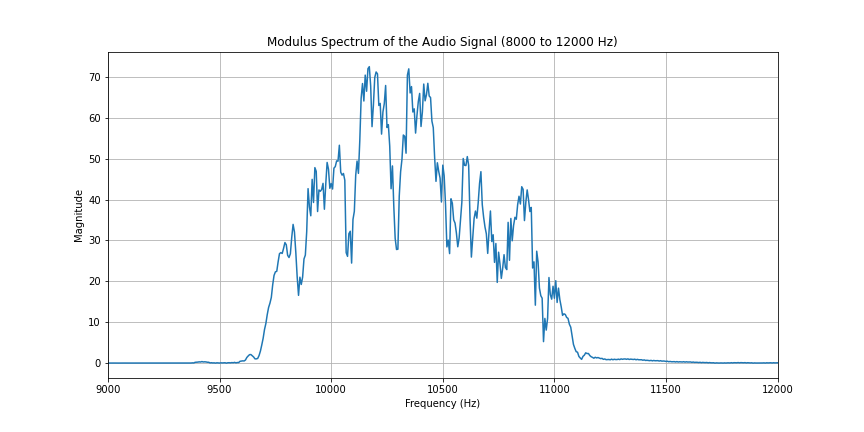
\includegraphics[width=1\textwidth]{modulus_spectrum.png}
\caption{Modulus spectrum of the bat signal.}
\end{figure}

In Figure 2, the spectrum is zoomed into the 9 kHz to 12 kHz range. This range is particularly interesting for bat signals as it contains key frequency components of their echolocation calls.

\subsubsection*{Identification of Frequency Components and Harmonics}
\begin{itemize}
    \item \textbf{Key Peaks:} The spectrum shows distinct peaks at specific frequencies, that are 9.75 kHz, 10.1 kHz, 10.25 kHz, and 10.4 kHz. These peaks are indicative of the signal's dominant frequency components.
        
    \item \textbf{Harmonics:} These subsequent peaks, appearing at regular intervals, are identified as the harmonics of the fundamental frequency. These harmonics are integral to the complex structure of the bat's echolocation signal. In the Fourier spectrum the harmonics are clearly shown, and the space between each peaks are evenly spaced for each subsequent peaks.
\end{itemize}

\begin{figure}[h]
    \centering
    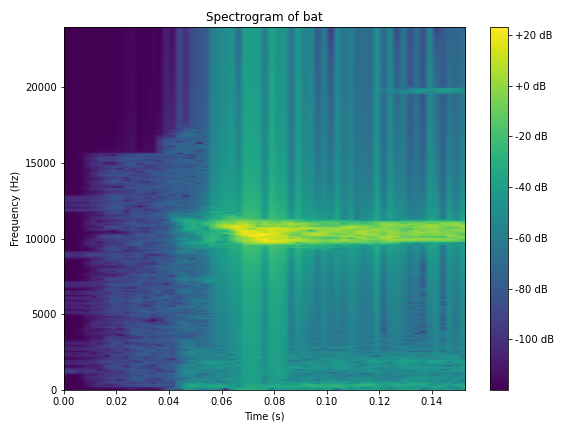
\includegraphics[width=0.8\textwidth]{spectrogram.png}
    \caption{Spectrogram of the bat sound.}
    \label{fig:spectrogram}
\end{figure}

\subsection{Spectrogram Analysis and Discussion (Q 3 - 4 and 3 - 5)}
The spectrogram of the bat signal was computed and analyzed to understand its frequency content over time. Here, the window duration is set to 0.01 seconds, with the Hamming window function to smooth out rough spots. Also, the frequncy of the bat is calculated by summing the energy across time for each frequency, and then identify the most prominent frequency. As the result, the frequency of the bat is approximately 10.157 kHz. The following observations were made based on the spectrogram plot:
\begin{itemize}
    \item \textbf{Presence and Variation of Frequencies: } The spectrogram reveals the presence of various frequency components at different times throughout the signal's duration. There is a particular interesting frequency at around 10 kHz to 11 kHz sharply evolve from 0.06 to 0.14 seconds. This is the frequency of the bat at around +20 bB from 0.06 to 0.08 seconds and sharply decreases to nearly +5 dB after.
    \item \textbf{Considerations of Shannon-Nyquist Criterion: }
        \begin{itemize}
            \item The spectrogram uses the sampling rate of \[f_s \geq 2 \cdot f_{\text{max}}\]
            \item After performing Fast Fourier Transform of the original sound, the sampling rate is at 48 kHz, and the maximum frequency in the signal is approximately 24 kHz.
        \end{itemize}
\end{itemize}
Given these observations, it appears that the Shannon-Nyquist criterion is satisfied in our analysis. While the criteria is met, this is just close enough to meet the Nyquist rate. So, any slight increase in the frequency content above 24 kHz could lead to aliasing. So, there should be the need for an anti-aliasing filter. So in practical applications, it's better to have a sampling rate significantly higher than the Nyquist rate. Still, for this analysis the choice of an appropriate sampling rate and the correct handling of the Nyquist frequency ensure that the spectrogram accurately represents the frequency content of the audio signal within the bounds of the provided sampling rate.

\subsection{Frequency Shifting and Time-Domain Analysis (Q 3 - 6)}
To observe the high-frequency oscillations of the bat signal in the time domain, a frequency shifting technique (heterodyning) is applied. This technique involves generating a sine wave at a specific frequency, multiplying it with the original signal, and then filtering the result with a low-pass filter.

\subsection*{Procedure}
\begin{itemize}
    \item A sine wave with a frequency of 11.5 kHz was generated and multiplied with the original bat signal. This step shifts the frequency content of the signal.
    
    \item A low-pass Butterworth filter with a cutoff frequency of 2 kHz is applied to the product of the signal and the sine wave. This filter isolated the downward-shifted component of the frequency spectrum.
\end{itemize}

\subsection*{Resulting Signal}
\begin{figure}[h]
\centering
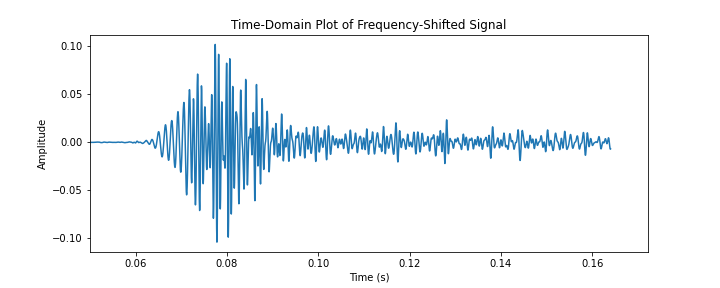
\includegraphics[width=1\textwidth]{shifted_time_domain.png}
\caption{Time-domain representation of the bat signal after frequency shifting.}
\end{figure}

The processed signal reveals oscillations that were not visible in the original high-frequency signal. The frequency shifting technique make oscillations in the time-domain signal more visible. The resulting time-domain plot exhibits a clean sine wave pattern from 0.05 to 0.1 seconds, with a peaked amplitude of 0.1 at approximately 0.080 seconds. This successful frequency shift has allowed us to clearly observe and analyze the oscillations. Additionally, this technique has proven effective in enhancing the interpretability of the data, contributing to a more comprehensive analysis.

\subsection{Classification (Q 3 - 7)}
Since the species of the bat is unknown, I will use Random Forests in this section to classify different species. This approach is chosen because there is only one parameter, which is the frequencies of the bat species. These frequencies demonstrate a non-linear relationship within the data, thus allowing for robust and accurate species classification. Subsequently, Support Vector Machines (SVM) will be used to predict the species of the unknown bat. A synthetic dataset, representing the echolocation frequencies of various bat species, was generated for analysis. This dataset was created to simulate the range of frequencies used by different bat species for echolocation. The following bat species were included in the dataset:
\begin{itemize}
    \item \textbf{Little Brown Bat (Myotis lucifugus):} frequency range from 20 kHz to 110 kHz.

    \item \textbf{Big Brown Bat (Eptesicus fuscus):} frequency range from 20 kHz to 60 kHz.

    \item \textbf{Mexican Free-tailed Bat (Tadarida brasiliensis):} frequency range from 25 kHz to 50 kHz.

    \item \textbf{Greater Horseshoe Bat (Rhinolophus ferrumequinum):} frequency range from 75 kHz to 110 kHz.

    \item \textbf{Lesser Horseshoe Bat (Rhinolophus hipposideros):} frequency range from 75 kHz to 110 kHz.

    \item \textbf{Soprano Pipistrelle (Pipistrellus pygmaeus):} frequency range from 55 kHz to 85 kHz.

    \item \textbf{Common Pipistrelle (Pipistrellus pipistrellus):} frequency range from 45 kHz to 70 kHz.

    \item \textbf{Spotted Bat (Euderma maculatum):} frequency range from 15 kHz to 50 kHz.
\end{itemize}


For each species, a set of 125 frequency values was generated, spanning their respective typical echolocation frequency ranges. These frequencies were synthesized based on known echolocation frequency ranges for each species and were uniformly distributed within these ranges.

The combined dataset, comprising all species, was then visualized using a scatter plot. In this plot, each point represents a frequency value for a particular bat species, with different species distinguished by unique colors. This visualization aids in understanding the distribution and range of frequencies utilized by each species.

\begin{figure}[ht]
\centering
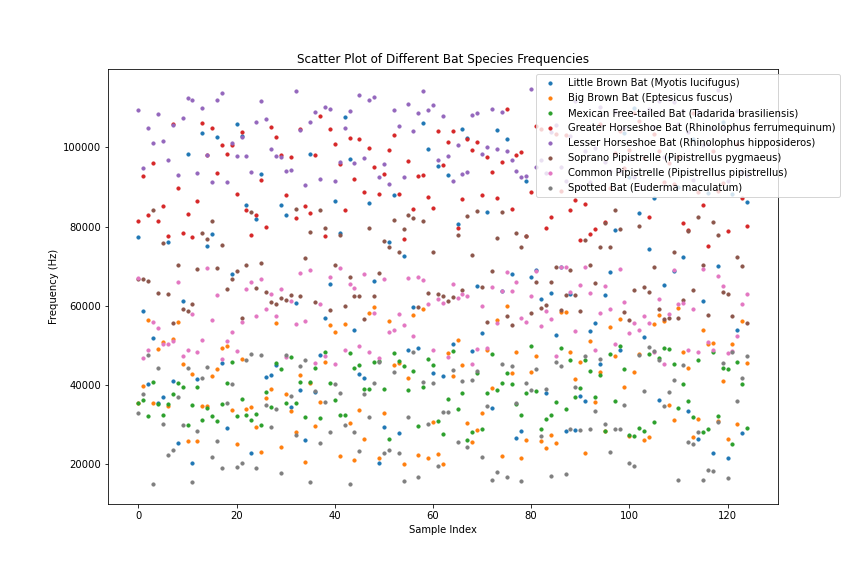
\includegraphics[width=1\textwidth]{bat_species_freq.png}
\caption{Scatter plot of synthetic bat species frequencies. Each color represents a different species, illustrating the variation in echolocation frequencies among them.}
\end{figure}

A Random Forest Classifier, an ensemble learning method, was employed for the classification of bat species based on frequency data. The classifier was configured with 500 decision trees and trained on a designated training dataset. Post-training, the model's efficacy was evaluated using a test dataset.

Classification report, encompassing metrics such as precision, recall, and F1-score for each class, alongside overall model accuracy.

\subsection{Classification Report}
The classification report provides a detailed assessment of the model's performance, including precision, recall, and F1-score for each species, as well as overall model accuracy.
\subsubsection{Analysis}
The analysis of the Random Forest Classifier's performance, as depicted in the classification report, provides several key insights:
\begin{center}
    \begin{tabular}{|c|c|c|c|c|}
    \hline
    Class & Precision & Recall & F1-Score & Support \\
    \hline
    0 & 0.25 & 0.22 & 0.23 & 24 \\
    1 & 0.54 & 0.56 & 0.55 & 27 \\
    2 & 0.43 & 0.42 & 0.43 & 24 \\
    3 & 0.79 & 0.70 & 0.75 & 27 \\
    4 & 0.27 & 0.26 & 0.26 & 27 \\
    5 & 0.24 & 0.35 & 0.29 & 17 \\
    6 & 0.50 & 0.62 & 0.55 & 26 \\
    7 & 0.68 & 0.54 & 0.60 & 28 \\
    \hline
    Accuracy & & & 0.47 & 200 \\
    \hline
    Macro Avg & 0.46 & 0.46 & 0.46 & 200 \\
    Weighted Avg & 0.48 & 0.47 & 0.47 & 200 \\
    \hline
    \end{tabular}
    \end{center}
    

\begin{itemize}
    \item \textbf{Overall Performance:} The classifier achieves an overall accuracy of 47\%, indicating a moderate level of effectiveness in species classification. This suggests that while the model is generally capable of distinguishing between species, there is still room for improvement.

    \item \textbf{Species-Specific Observations:}
    \begin{itemize}
        \item Species 1, 2, and 4 show a reasonable balance between precision and recall, suggesting a relatively reliable performance in these classes.
        \item Species 3 and 7 exhibit high precision and recall, indicating a high level of accuracy in classifying these species.
        \item Conversely, species 0, 4 and 5 demonstrate lower precision and recall, highlighting potential challenges the model faces in accurately classifying these particular species.
    \end{itemize}
    \item \textbf{Implications for Model Improvement:} The discrepancies in performance across different species suggest a need for further model tuning, possibly through hyperparameter optimization, or exploring alternative feature sets. Additionally, addressing any imbalance in the training data could enhance the model's ability to accurately classify underrepresented species. Furthermore, since the datasets only include the frequencies of each species, it's very hard for the algorithms to perform classification due to limitations in parameters. To improve this model, more parameters can be included such as, wing span, weights, and size of each species to perform better classification.
\end{itemize}


\subsection*{Identification of bat species}
\section{Analysis of SVM Classification Probabilities}

The Support Vector Machine (SVM) classifier was employed to predict the likelihood of an unknown bat frequency belonging to each known bat species. The probabilities represent the model's confidence in classifying the unknown frequency into each species category.

\subsection{Probability Distribution}
The following table showcases the probability distribution as predicted by the SVM model for each species:

\begin{center}
\begin{tabular}{lr}
\toprule
Species & Probability \\
\midrule
Big Brown Bat (Eptesicus fuscus) & 0.244 \\
Common Pipistrelle (Pipistrellus pipistrellus) & 0.007 \\
Greater Horseshoe Bat (Rhinolophus ferrumequinum) & 0.014 \\
Lesser Horseshoe Bat (Rhinolophus hipposideros) & 0.009 \\
Little Brown Bat (Myotis lucifugus) & 0.166 \\
Mexican Free-tailed Bat (Tadarida brasiliensis) & 0.029 \\
Soprano Pipistrelle (Pipistrellus pygmaeus) & 0.024 \\
Spotted Bat (Euderma maculatum) & 0.505 \\
\bottomrule
\end{tabular}
\end{center}

\subsection{Discussion of Results}
The SVM model demonstrates a decent probability (approximately 50.5\%) for the unknown bat frequency being classified as a Spotted Bat (Euderma maculatum), the other candidates are Big Brown bat (Eptesicus fuscus) (approximately 24.4\%) and Little Brown Bat (Myotis lucifugus) (approximately 16.6\%). This probability suggests a decent confidence by the model in this classification, potentially indicating frequency characteristics resemblance to the Spotted Bat that are captured by the SVM classifier.

In contrast, the probabilities associated with the rest relatively low, mostly around 1\%. This disparity in probabilities indicates that the frequency characteristics of the unknown bat sound are most closely aligned with those typically attributed to the Spotted Bat (no. 1) Big Brown bat (no. 2) and Little Brown Bat (no. 3), as compared to other species in the dataset. \footnote{Code is in \href{https://github.com/hoang-nguyen13/Bat_Sound.git}{Github.}}


\section{Conclusion}

\subsection{Project Overview}
The project involved understanding the time-domain signal, performing Fourier transforms, and generating spectrograms of the original sound. This sound analysis provided insights into the frequency of the unknown bat. These techniques help identifying the frequency of the unknown bat, so machine learning techniques were then applied to classify different bat species to search for the species of the unknown bat, which in this case, it's likely to be Eptesicus fuscus (with 50.5\% probability).
\subsection{Machine Learning Application}
Two machine learning models — Support Vector Machine (SVM), Random Forest — were employed to classify bat species based on their frequencies. However, the classification accurate rate is moderate due to limiting parameter that is the species frequency, further improvement in classification can be conducted with additional parameters such as species' weight and winspans.
\subsection{Insights and Future Directions}
This study motivates the diversification and exploration of new bat species and their use of echolocation. Through the categorization of intrinsic properties such as frequency, machine learning proves to be a valuable tool in wildlife research, particularly for the classification and study of bioacoustic data. While the models are effective, they also reveal areas for improvement, including dealing with overlapping frequency ranges and enhancing model accuracy for specific species. Future endeavors could expand upon this work by incorporating additional acoustic features, exploring more advanced machine learning algorithms, and applying the models to real-world echolocation data. Such advancements could significantly contribute to conservation efforts and enhance our ecological understanding of bats.
\end{document}

